\documentclass[journal, a4paper]{IEEEtran}

\usepackage[hidelinks]{hyperref}  % PDF Hyperlinks


\usepackage{lipsum}               % Lorem Ipsum


\usepackage{siunitx}              % SI Units
\usepackage{booktabs}             % Tables
\usepackage{caption}              % Captions


\usepackage{graphicx}             % Images or Graphics
\usepackage{pgfplots}             % Graphs and Plots

\usetikzlibrary{mindmap}
\usetikzlibrary{positioning}


% correct bad hyphenation here
\hyphenation{op-tical net-works semi-conduc-tor}


\begin{document}
\title{A Literature Review on NDT and SHM}


% === Authors === %
\author{Antonette~C.~Maxey,~\IEEEmembership{CPE Student,~MMCM,}
        Florencio~N.~Pulido,~\IEEEmembership{CPE Student,~MMCM,}
        and~Vincent~Alfred~B.~Tomas,~\IEEEmembership{ECE Student,~MMCM}% <-this % stops a space
}



% The paper headers
\markboth{Methods of Research Literature Review, February~2024}%
{Shell \MakeLowercase{\textit{et al.}}: Developing a Portable NDT Device for Efficient SHM}


% === Build Title Area  === %
\maketitle


\begin{abstract}
  This literature review focuses on the advancements and challenges in Structural Health Monitoring (SHM)
  through the lens of portable Non-Destructive Testing (NDT) devices.
  These devices offer promising solutions to the limitations of traditional SHM methods, such as high cost and complexity.
  This review encompasses various aspects including existing portable NDT devices, sensor technology,
  data acquisition and analysis, as well as applications and case studies. It identifies significant advancements
  in sensor technologies and data analytics for NDT and SHM, while also highlighting critical limitations and research gaps.
  The synthesis and critique section emphasize the need for improvements in sensor accuracy, data processing capabilities,
  and environmental robustness for optimal infrastructure safety. Future developments in portable NDT devices are seen
  in the integration of advanced technologies like embedded systems, wireless sensors, cloud computing, and artificial intelligence.
  The findings underscore the importance of addressing these challenges for the successful deployment of portable NDT
  devices in SHM applications, paving the way for enhanced efficiency and accessibility in ensuring structural integrity.
\end{abstract}


% Note that keywords are not normally used for peerreview papers.
\begin{IEEEkeywords}
  NDT, SHM, Portable.
\end{IEEEkeywords}







\section{Introduction}
\IEEEPARstart{S}{tructural} Health Monitoring (SHM) is a pivotal engineering tool, providing real-time structural integrity data,
thereby ensuring safety and averting infrastructure failures \cite{Gharehbaghi2022} \cite{Katam2023}.
Traditional SHM methods, while effective, are often limited by factors such as
high cost, complexity, and accessibility issues \cite{Katam2023} \cite{Gharehbaghi2022}.
A portable, Non-Destructive Testing (NDT) device presents a promising solution for efficient and accessible SHM,
overcoming the limitations of traditional methods \cite{Guo2022} \cite{Chen2023}.
The objective of this capstone project is to explore the potential of a portable,
NDT device in overcoming the limitations of traditional SHM methods.

SHM is a field dedicated to the ongoing monitoring and evaluation of the structural integrity
of various infrastructure systems \cite{Katam2023}, NDT is a method that enables the assessment
of structural degradation without causing actual damage to the structure itself \cite{Katam2023},
and a portable NDT device is a tool that enhances the efficiency and accessibility of SHM \cite{Hassani2023} \cite{Katam2023}.
Various NDT methods, each with its unique advantages and disadvantages,
offer diverse approaches to assessing structural integrity without causing damage \cite{Dolati2021} \cite{Verma2013}.
Existing portable NDT devices, while offering promising functionalities,
also present certain limitations that need to be addressed for optimal SHM \cite{Hassani2023} \cite{Zhu2011}.
Relevant theories and frameworks related to structural safety, damage detection,
and sensor technology play a crucial role in enhancing the effectiveness of SHM
and ensuring the safety of various infrastructures \cite{Chen2021} \cite{Gharehbaghi2022}.


\section{Methodology}
\lipsum[3]

\begin{figure}
  \centering
  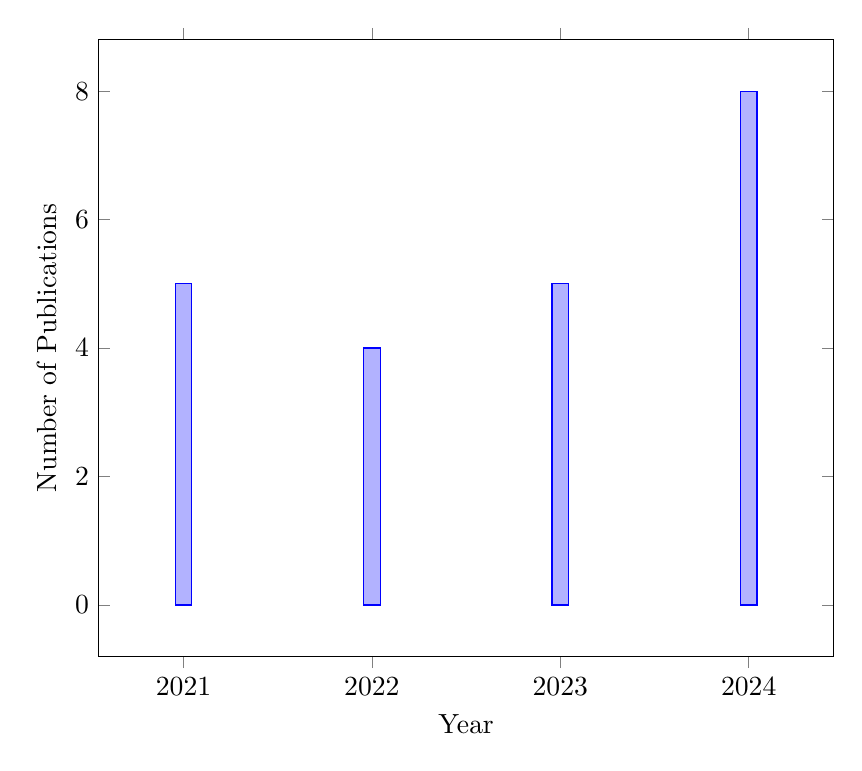
\begin{tikzpicture}
    \begin{axis}[
        ybar,
        width=0.9\columnwidth,                                          % Adjust the width of the plot
        bar width=6pt,                                                  % Adjust the width of the bars
        xlabel={Year},                                                  % Label for the x-axis
        ylabel={Number of Publications},                                % Label for the y-axis
        xtick=data,                                                     % Use data points as x-axis labels
        xticklabels={2021, 2022, 2023, 2024},                           % Labels for the x-axis ticks
        ymin=0,                                                         % Set the minimum value for the y-axis
        enlarge x limits=0.15,                                          % Add space to the left and right of the x-axis
        enlarge y limits=0.1,                                           % Add space to the top and bottom of the y-axis
        legend style={at={(0.5,-0.15)},anchor=north,legend columns=-1},
      ]
      \addplot coordinates {(2021, 5)  (2022, 4)  (2023, 5) (2024, 8)};
    \end{axis}
  \end{tikzpicture}
  \caption{Number of Publications Over the Years}
  \label{fig:publications}
\end{figure}

\lipsum[1]


\section{Results and Discussion of Scientometric review}
\lipsum[1]


\subsection{Analysis of Journals}
As shown in \autoref{tbl:bibliometricRanking} \lipsum[1]


\begin{table}[htbp]

  \centering
  \caption{Bibliometric Ranking Of Journals}
  \label{tbl:bibliometricRanking}
  \begin{tabular}{lcc}

      \toprule
      \textbf{Journal} & \textbf{No. of Documents} & \textbf{No. of Citations} \\
      \midrule
      Journal of San                   & 1     & 602   \\
      Journal of Hon                   & 1     & 100   \\
      Heh Periodicals                  & 1     & 195   \\
      Sensors in thw World             & 1     & 515   \\
      \bottomrule
  \end{tabular}
\end{table}

It is evident in \autoref{tbl:bibliometricRanking} \lipsum[1]


\subsection{Active Researchers}
As seen in \autoref{tbl:bresearchers} \lipsum[1]

\begin{table}[htbp]

  \centering
  \caption{Top Researchers}
  \label{tbl:bresearchers}
  \begin{tabular}{lccc}

      \toprule
      \textbf{Author} & \textbf{Documents} & \textbf{Citations} & \textbf{TLS} \\
      \midrule
      Hasan A.                   & 1     & 602   &  31         \\
      Rodulf K. A.               & 1     & 100   &  11         \\
      Libre F. C.                & 1     & 195   &  18         \\
      Gigometre S.               & 1     & 515   &  7          \\
      \bottomrule
  \end{tabular}
\end{table}

However, it shall be noted that \autoref{tbl:bresearchers} \lipsum[1]\lipsum[1]


\subsection{Article Sitation Analysis}
It is imperative as shown in \autoref{tbl:articleCites} \lipsum[1]

\begin{table}[htbp]

  \centering
  \caption{Top-Cited Articles}
  \label{tbl:articleCites}
  \begin{tabular}{lcc}

      \toprule
      \textbf{Article} & \textbf{No. of Citation} \\
      \midrule
      Author Name       \cite{Hu2023}           &    331         \\
      Rodulf K. A.      \cite{Lingxin2022}      &    141         \\
      Libre F. C.       \cite{Entezami2020}     &    118         \\
      Gigometre S.      \cite{Lee2023}          &    71          \\
      \bottomrule
  \end{tabular}
\end{table}

Hence, the data in \autoref{tbl:articleCites} \lipsum[1]



\subsection{Keyword Analysis}
That the closer as show in \autoref{fig:co_occurrence} \lipsum[1]

\begin{figure}[htbp]
  \centering
  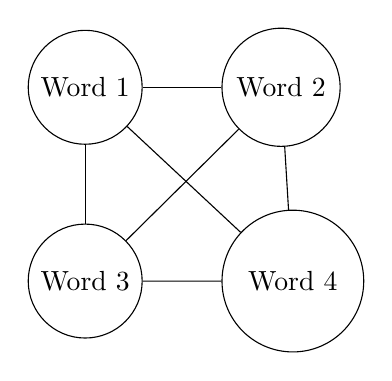
\begin{tikzpicture}[scale=0.8]
    \node[circle,draw,minimum size=1cm] (word1) at (0,0) {Word 1};
    \node[circle,draw,minimum size=1.5cm] (word2) [right=of word1] {Word 2};
    \node[circle,draw,minimum size=1.2cm] (word3) [below=of word1] {Word 3};
    \node[circle,draw,minimum size=1.8cm] (word4) [right=of word3] {Word 4};
    
    \draw (word1) -- (word2);
    \draw (word1) -- (word3);
    \draw (word1) -- (word4);
    \draw (word2) -- (word3);
    \draw (word2) -- (word4);
    \draw (word3) -- (word4);
  \end{tikzpicture}
  \caption{Co-occurrence Network of Words}
  \label{fig:co_occurrence}
\end{figure}

However, unlike with \autoref{fig:co_occurrence} \lipsum[1]






\section{Results and Discussion of Systematic Review}

\subsection{Existing Portable NDT Devices}
Recent research and development efforts have led to significant advancements in portable NDT devices
for SHM applications \cite{Vijayan2023} \cite{Parsy2018} \cite{Hassani2023}.
Various devices, each with their unique functionalities, target applications, and performance characteristics,
have been analyzed to understand their potential in different fields \cite{Khanna2020} \cite{Baig2021} \cite{Corzo2020}.
Existing research has identified several limitations and challenges, such as sample characteristic limitations,
methodological limitations, psychometric limitations, and qualitative research limitations.


\subsection{Sensor Technology for SHM}
Recent advancements in sensor technology, such as miniaturization, low-power consumption, and wireless communication,
have significantly enhanced the capabilities of portable NDT devices,
making them more efficient and accessible for SHM applications \cite{Hassani2023} \cite{Valeske2020}.
The integration of different sensor types and their data fusion approaches is crucial
for comprehensive SHM, as it allows for a more accurate\
and holistic assessment of structural integrity \cite{Broer2022} \cite{Azimi2020}.
Sensor technology limitations, such as accuracy, precision, and robustness,
can significantly impact the performance and reliability of devices,
necessitating further research and development in this area \cite{Varshney2021} \cite{Moore2020}.


\subsection{Data Acquisition and Analysis for SHM}
Methods for data acquisition, processing, and analysis from portable NDT
devices have seen significant advancements, with research highlighting the use of optical
and electrochemical methods for in situ detection of trace heavy metal ions \cite{Hu2023}.
Approaches for real-time data monitoring, damage detection algorithms, and data visualization techniques
are integral to the effective application of SHM, with advancements in these areas
significantly enhancing the capabilities of portable NDT devices \cite{Azimi2020} \cite{Lingxin2022}.
Efficient SHM decision-making is often challenged by issues related
to data management and interpretation, such as the complexity of handling big data and the time-consuming procedures
for feature extraction and statistical decision-making \cite{Entezami2020}.


\subsection{Applications and Case Studies}
Portable NDT devices have been successfully applied in various SHM
scenarios, including bridges, buildings, and industrial structures, demonstrating their versatility and effectiveness \cite{Parsy2018} \cite{Azimi2020}.
The cost-effectiveness, ease of use, and reliability of portable NDT
devices in real-world settings have been demonstrated, with the modularized structure of the device offering
cost-effectiveness through the reusability of high-cost modules and enhancing convenience by eliminating the
necessity for multiple separate monitoring devices \cite{Lee2023}.
Emerging trends in portable NDT technology for SHM
include the integration of intelligent technologies such as the Internet of Things (IoT), Artificial Intelligence (AI),
and advancements in sensor technologies, which have led to remarkable improvements in SHM for various applications
including residential, commercial, industrial, historical, and special buildings \cite{Vijayan2023} \cite{Hassani2023}. 


\subsection{Synthesis and Critique}
The literature review reveals significant advancements in sensor technologies and data analytics
for NDT and SHM,
while also highlighting limitations and research gaps that need to be addressed for optimal infrastructure safety \cite{Vijayan2023} \cite{Hassani2023}.
Existing portable NDT devices have shown effectiveness in SHM,
however, their performance can be influenced by factors such as sensor accuracy, data processing capabilities,
and environmental conditions \cite{Vijayan2023} \cite{Hassani2023}.
Opportunities for improvement and future development in portable NDT devices
for SHM lie in the integration of advanced technologies such as embedded systems,
wireless sensors, cloud computing, and artificial intelligence for improved analytics, error-free inference,
and efficient troubleshooting \cite{Meier2018}.


\section{Discussion and Future Directions}  %  Discussion and future directions
The research question of this capstone project is to explore the potential of a portable,
NDT device in overcoming the limitations of traditional SHM methods,
and the literature review reveals significant advancements in sensor technologies and data analytics for NDT and SHM,
while also highlighting limitations and research gaps that need to be addressed for optimal infrastructure safety.
The findings from the literature review have significant implications for the development of the
proposed portable NDT device, highlighting the need for advancements in sensor technologies,
data analytics, and overcoming limitations and research gaps for optimal infrastructure safety \cite{Udell2018} \cite{Meier2018}.
The next steps in this capstone project involve the design and development of a portable
NDT device, with considerations for sensor selection, data acquisition and processing methods,
and the expected outcomes include improved efficiency and accessibility in SHM.





\section*{Acknowledgment}
The authors would like to thank \lipsum[1]



% Can use something like this to put references on a page
% by themselves when using endfloat and the captionsoff option.
\ifCLASSOPTIONcaptionsoff
  \newpage
\fi


% === Bibliography ===

\bibliographystyle{IEEEtran}
\bibliography{bibtex/bib/references}

% === End of Bibliography ===


\end{document}


